
\documentclass{article}
\usepackage{amsmath, amsfonts, amssymb, amsthm} %packages for math-related
\usepackage[margin=1.2in]{geometry}
\usepackage[shortlabels]{enumitem}
\usepackage[utf8]{inputenc}
\usepackage{graphicx} % package for inserting images
\usepackage{commath} % package for things like \del, \cbr, and \sbr. These handle parentheses well.
\usepackage[mathscr]{euscript}%for \scr command 
\usepackage{../commands} %package with all of the commands for this class
\usepackage{url}
\setlength{\parindent}{0em} % so paragraphs aren't indented
\newcommand{\lcm}{\text{lcm}}
\newcommand{\Hom}{\text{Hom}}
\newcommand{\Ann}{\text{Ann}}
\newcommand{\Cc}{{C_c^\infty(\RR)}}
% ********************************************************** %
%               THINGS TO EDIT BELOW THIS LINE               %
% ********************************************************** %
\newcommand{\D}{\nabla}
\renewcommand{\d}{\partial}
\usepackage{wrapfig}
\title{\textsc{MATH 173 Problem Set 3}}
\author{Stepan (Styopa) Zharkov}
\date{April 20, 2022}
\begin{document}
\maketitle
\problem{1}Show that the only solution $u \in \cal{D}'(\RR)$ of $u' = 0$ is $u = c$, where $c$ is a constant function. \tri
\hop
\solution
As the hint suggests, $u' = 0$ means by definition $u(\phi) = 0$ for any $\phi \in C_c^\infty(\RR)$. For any $\psi \in \Cc$, let $\phi_0\in \Cc$ be a bump function such that $\int_\RR \phi_0(x)dx = 1$. Let $\hat{\psi} = \psi - \phi_0\int_\RR\psi(x)dx$. We see that 
\[\int_\RR \hat{\psi}(x)dx = \int_\RR \psi(x)dx -\int_R\psi(x)dx\cdot \int_\RR\phi_0(x)dx =\int_\RR \psi(x)dx-\int_\RR \psi(x)dx = 0.\]
So, we can let 
\[\phi(x) = \int_{-\infty}^x \hat{\psi}(x) dx.\]
We see $\hat{\psi}$ has compact support and is in $\Cc$ (since it is the sum of two compact support functions). Since $\int_\RR \hat{\psi}(x)dx = 0$, we know $\phi$ must have compact support as well and be in $\Cc$. Now, let $c = u(\phi_0)$. We see that by linearity of $u$,
\[u(\psi) = u(\hat{\psi}) + u(\phi_0)\cdot \int_\RR\psi(x)dx = u(\phi') + c\int_\RR\psi(x)dx =0+  c\int_\RR\psi(x)dx=c\int_\RR\psi(x)dx, \]
which is exactly what we wanted to prove. 
\qed


\newpage
\problem{2} Let $f \in \cal{D}'(\RR)$, define a solution $u \in \cal{D}'(\RR^2)$ such that $u_t +cu_x = 0$ and $u(t,x) = f(x-ct)$ in the sense of distributions.
\tri
\hop
\solution
First, let us define $f(x-ct)$ in a way that aligns with the case that $f$ is a nice function. We see that if $f$ were nice, then
\begin{align*}
    f(x-ct)(\phi)&= \int_{\RR^2}f(x-ct)\phi(t,x)dxdt \\
    &= \int_{\RR^2}f(z)\phi(s,z+cs)dzds \\
    &= \int_{\RR^2}f(z)\phi(s,z+cs)dsdz \\
    & = \int_{z \in \RR} f(z) \int_{s \in \RR} \phi(s,z+cs)ds dz\\
    &= f\del{\int_{s \in \RR}\phi(s,z+cs)ds}. 
\end{align*}
So, we see that $f(x-ct)(\phi) = f(\Phi)$ where $\Phi = \int_\RR \phi(s,z+cs)ds$. Note that $\Phi \in \Cc$ because the integral of a smooth function is smooth and $\phi$ is compactly supported. So, we can define $u = f(x-ct)$. 
\hop 
Now, we must show that $u$ satisfies the PDE. This is done by simply writing out our definition and using the linearity of $f$. More precisely, 
\begin{align*}
    (u_t + cu_x)(\phi) &= -f\del{\int_s \phi_t(s, z +cs) ds} -cf\del{\int_s \phi_x(s, z +cs) ds} \\
    &= -f\del{\int_s \sbr{\phi_t(s, z +cs) +s\phi_x(s, z +cs)} ds} \\
    & = -f\del{\int_s\d_s \phi(s,z+cs) ds)}\\
    &= -f(0) \\
    &= 0.
\end{align*} 
Note that we used the fundamental theorem of calculus, that $\phi$ has compact support, and that $f$ is linear in the above computation. 
\hop 
Thus, $u = f(x-ct)$ by definition and $u$ solves the PDE in the sense of distribution, as we wanted to show.
\qed


\newpage
\problem{3} \begin{enumerate}[(a)]
    \item Find the general $C^2$ solution of the PDE $u_{xx} - u_{xt} - 6u_{tt} = 0$ by reducing it to a
    system of first order PDEs.
    \item Show that if $f,g \in \cal{D}'(RR)$, and we define new distributions $v,w \in \cal{D}'(\RR^2)$ similar to Problem 2,
    such that formally $v(x,t) = f(3x+ t), w(x,t) = g(2x- t)$, then $u = v + w$ solves the PDE in part (a).
\end{enumerate}
 \tri
\hop
\solution
\begin{enumerate}[(a)]
    \item This part follows directly from what we have done in class. We can factor 
    \[u_{xx}-u_{xt}-6u_{tt} = (\d_x - 3\d_t)(\d_t + 2\d_t)u,\]
    so the general $C^2$ solution is 
    \[u(x,t) = g(2x-t) + f(3x + t)\]
    for some $C^2$ functions $f,g$. \qed
    \item This problem is similar to problem 2, but here we should apply a trick instead of mindlessly taking derivatives. We will split up $ (\d_x - 3\d_t)(\d_t + 2\d_t)$ and apply them to the parts of $u$ in different orders. More precisely, we see that 
    \begin{align*}
        (\d_x - 3\d_t)(\d_t + 2\d_t)u &= (\d_x - 3\d_t)(\d_t + 2\d_t)( g(2x-t) + f(3x + t)) \\ 
        &= (\d_t + 2\d_t)(\d_x - 3\d_t)f(3x + t) +  (\d_x - 3\d_t)(\d_t + 2\d_t)g(2x-t).
    \end{align*}
    By a similar derivation to that in problem 2, we can define 
    \[f(3x+t)(\phi) = f\del{\frac{1}{3}\int_s \phi(s, (z-s)/3)ds}\]
    and 
    \[g(2x-t)(\phi) = g\del{\frac{1}{2}\int_s \phi(s, (z+s)/2)ds}\]
    Now, we see that 
    \begin{align*}
        (\d_t + 2\d_t)(\d_x - 3\d_t)f(3x + t)(\phi) &= (\d_t + 2\d_t)(\d_x - 3\d_t)f\del{\frac{1}{3}\int_s \phi(s, (z-s)/3)ds} \\
        &=-(\d_t + 2\d_t)f\del{\int_s \sbr{\frac{1}{3}\phi_x(s, (z-s)/3) - \phi_t(s, (z-s)/3)}ds}\\
        &= -(\d_t + 2\d_t)f\del{\int_s \d_s \phi(s, (z-s)/3)ds} \\
        &= -(\d_t + 2\d_t)f(0)\\
        &= -(\d_t + 2\d_t)0\\
        &=0,
    \end{align*}
    where we used the fundamental theorem of calculus along with the fact that $\phi$ must have compact support. 
    \hop 
    Similarly,
    \begin{align*}
        (\d_x - 3\d_t)(\d_t + 2\d_t)g(2x - t)(\phi) &= (\d_x - 3\d_t)(\d_t + 2\d_t)g\del{\frac{1}{2}\int_s \phi(s, (z+s)/2)ds} \\
        &=-(\d_t - 3\d_t)g\del{\int_s \sbr{\frac{1}{2}\phi_x(s, (z+s)/2) + \phi_t(s, (z-s)/2)}ds}\\
        &= -(\d_t - 3\d_t)g\del{\int_s \d_s \phi(s, (z+s)/2)ds} \\
        &= -(\d_t - 3\d_t)f(0)\\
        &= -(\d_t -3\d_t)0\\
        &=0,
    \end{align*}
    where, again, we used the fundamental theorem of calculus along with the fact that $\phi$ must have compact support. 
    \hop 
    From this, we can conclude that 
    \begin{align*}
        u_{xx}-u_{xt}-6u_{tt} = (\d_t + 2\d_t)(\d_x - 3\d_t)f(3x + t) +  (\d_x - 3\d_t)(\d_t + 2\d_t)g(2x-t) = 0+0 = 0.
    \end{align*}
    So $v+w$ does indeed solve the PDE in part (a). \qed
\end{enumerate}


\newpage
\problem{4} Solve the equation $u_{xx} + 3u_{xy} - 4u_{yy} = 0, u(x,x) = \sin x, u_x(x,x) = 0$. \tri
\hop
\solution This problem can be solved using the standard method for second order hyperbolic PDEs of two variables with constant coefficients that we saw in class. 
\hop 
First, we can factor 
\[u_{xx} + 3u_{xy} -4u_{yy} = (\d_x - \d_y)(\d_x + 4\d_y)u.\]
So, as we know, the general solution has the form 
\[u(t,x) = f(4x - y)+ g(x+y).\]
Now, we just need to use the initial conditions to find the specific $f$ and $g$. We see that 
\[f(3x)+g(2x) = \sin x\]
and that 
\[4f'(3x) + g'(2x) = 0.\]
Taking the derivative of the former gives us that 
\[3f'(3x)+2g'(2x) = \cos x.\]
Now, we have a system of linear equations, so we can solve to see that 
\[3f'(3x) = - \frac{3}{5}\cos x \text{ and } g'(2x) = \frac{8}{5} \cos x .\]
Since $f(3x) + g(2x) = \sin x$, the constant during integration must be the same, so we can assume it to vanish and
\[f(x) = -\frac{3}{5}\sin(x/3) \text{ and } g(x) = \frac{8}{5}\sin(x/2).\]
Plugging this back in, we see that 
\[u(x,t) =  -\frac{3}{5}\sin\del{\frac{4x-y}{3}} + \frac{8}{5}\sin\del{\frac{x+y}{2}},\]
which is the solution we were after. \qed


\newpage
\problem{5} Solve the wave equation $u_{tt} -c^2u_{xx} = 0, u(x,0) = \phi(x), u_t(x,0) = \psi(x)$,
\[\text{with } \phi(x) = \begin{cases}
    0, x < -1, \\
    1 + x, -1 < x < 0,\\
    1 - x, 0 < x < 1,\\
    0, x >1, 
\end{cases} \text{ and } \psi(x) = \begin{cases}
    0, x < -1, \\
    2, -1 < x < 1,\\
    0, x > 1.
\end{cases}\]
Also describe where the solution vanishes and where it is $C^\infty$. You can assume $c=1$ for this. 
\tri
\hop
\solution
First, lets' consider the case $c =0$. Then, we have $u_{tt} = 0$, so $u_t(x,t)$ is constant along the line $\{(t,x_0)\}$ for any $x_0$. So, $u(t,x)$ has is a line of constant slope along any $\{(t,x_0)\}$. The starting point and the slope are defined by the initial conditions, so we see that 
\[u(t,x) = \phi(x) + t\psi(x).\]
This vanishes when $\phi(0) + t\psi =0$. Since $\phi, \psi$ are positive, $\phi$ must be $0$, so $|x| \ge 1$. Any point where $|x| \ge 1$ works. 
\hop 
We can also check that $u$ is linear (and thus $C^\infty$) everywhere except for the places where of $\phi$ and $\psi$ are not $C^\infty$. In other words $u$ is $C^\infty$ when $x \ne -1,0,1$. 
\hop
Now, let's look at the nonzero case. We know from the notes that the solution is 
\[u(t,x) = \frac{1}{2}(\phi(x+ct) + \phi(x-ct)) + \frac{1}{2c}\int_{x-ct}^{x+ct}\psi(\sigma) d\sigma.\]
Notice that we can assume $c > 0$ because $c < 0$ would also flip the integral, leading to the same solution. 
\hop 
We see that $\phi, \psi$ are non-negative, so this vanishes only when $\phi(x-ct)=0, \phi(x+ct)=0$, and $\psi = 0$ on the interval $(x-ct,x+ct)$. For the analysis of when $u$ vanishes, we will only consider $c =1$. We see that this is true when $[x-ct,x+ct] \cap (-1,1) = \varnothing$.  Instead of writing out the cases, consider the following picture of where this is true:

\begin{center}
    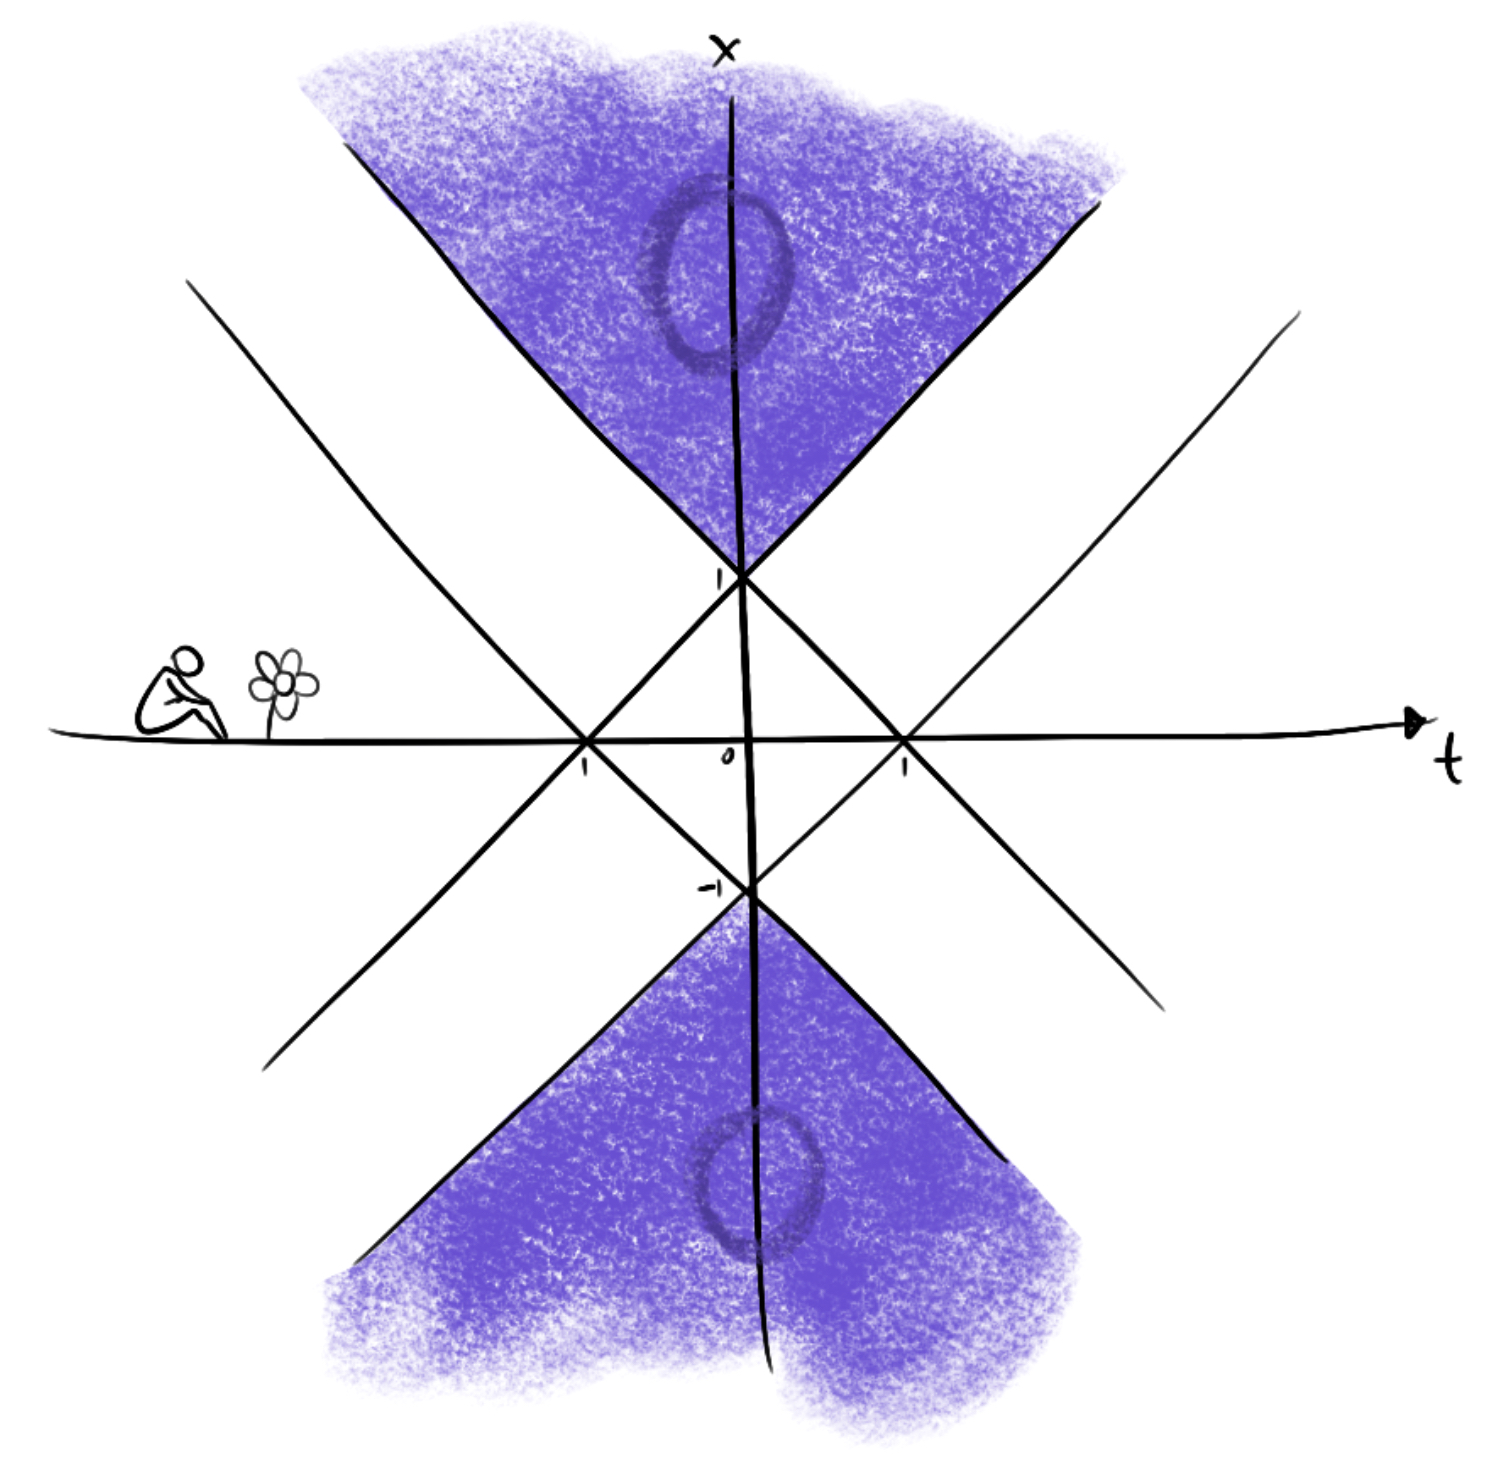
\includegraphics[height=7cm]{../images/0void1.jpeg}
\end{center}

We see that $u$ is $C^\infty$ everywhere but the discontinuities of $\phi, \psi$. In other words, $u$ is $C^\infty$ when $x+ct \ne -1, 0$, or 1. \qed


\newpage
\problem{6} Consider the wave equation on $\RR^n: u_{tt} - c^2\D_xu = f, u(x,0) = \phi(x),u_t(x,0) = \psi(x)$, and
write $x = (x_0,x_n)$ where $x_0 = (x_1,\dots,x_{n-1})$. Show that if $f(x_0,x_n,t) = f(x_0,- x_n,t), \phi(x_0,- x_n) =
\phi(x_0,x_n)$, and $\psi(x_0,-x_n) = \psi(x_0,x_n)$ for all $x$ and $t$, then $u(x_0, x_n, t) = u(x_0, -x_n, t)$.
\hop
i.e. if $f, \phi$ and $\psi$, are all even functions of $x_n$,
then $u$ is an even function of $x_n$ as well. \tri
\hop
\solution
As the hint suggests, consider $v(x_0, x_n, t) = u(x_0, x_n, t) - u(x_0, -x_n, t)$. Notice that 
\begin{align*}
    v_{tt} - c^2\Delta_xv &= u_{tt}(x_0, x_n, t) - u_{tt}(x_0, -x_n, t) - c^2\Delta_{x}u(x_0, x_n, t) + c^2\Delta_{x}u(x_0, -x_n, t)\\
    & = f(x_0, x_n, t) - f(x_0, -x_n, t)\\
    &= 0.
\end{align*}
We also see that 
\[v(x, x_n, 0) = u(x_0, x_n,0) - u(x_0, -x_n, 0) = \phi(x_0, x_n) - \phi(x_0, -x_n)=0\]
and 
\[v_t(x, x_n, 0) =u_t(x_0, x_n,0) - u_t(x_0, -x_n, 0) = \psi(x_0, x_n) - \psi(x_0, -x_n)=0. \]
So, $v$ solves the equation $v_{tt} - c^2\Delta_xv = 0$ with 0 initial conditions. By the uniqueness in the notes, we know that the only solution to this is $v=0$. Thus, we see that $u(x_0, x_n, t) - u(x_0, -x_n, t) = v(x_0, x_n, t) = 0$, so 
\[u(x_0, x_n, t) = u(x_0, -x_n, t),\]
and $u$ is even with respect to $x_n$, exactly as we wanted. 
\qed


\newpage
\problem{7} In this problem we prove the finite speed of propagation for solutions of variable coefficient wave equation. Consider the PDE $u_{tt} - \D \cdot (c^2\D u) + qu = 0, u(x,0) = \phi(x), u_t(x,0) = \psi(x)$,
where $c > 0$ and $q  \ge 0$ , depend on $x$ only, and $c$ is bounded between two positive constants, i.e., for
some $c_1,c_2 > 0, c_1 \le c(x) \le c_2$ for all $x \in \RR^n$. Assume that $u$ is a $C^2$ solution. You can assume $n= 1$ for this problem.
\begin{enumerate}[(a)]
    \item  Fix $x_0 \in \RR^n$ and $R_0 > 0$, and for $t < R_0/c_2$ let
    \[E(t) =\int_{\Omega(t)}(u_t^2 + c(x)^2|\D u |^2 + q(x)u^2) dx\]
    Show that $E$ is non-increasing in $t$. 
    \item Suppose that $\phi$ and $\psi$ satisfy $\phi(x) = \psi(x) = 0$ when $|x| > R$. Show that $u(t,x) = 0$ when
    $|x|> R + c_2t$.
    \item Prove that there is at most one $C^2$ solution in $[0,t_0] \times \RR^n$.
\end{enumerate}
\tri
\hop
\solution
\begin{enumerate}[(a)]
    \item For this problem, we will show that the derivative of $E$ is never positive. Let $\Omega(t)$ be the region where $|x-x_0| < R_0 - c_t$. We see that the product rule gives us that 
    \begin{align*}
        E'(t) &= \d_t \int_{\Omega(t)}(u_t^2 + c(x)^2|\D u |^2 + q(x)u^2) dx \\
        &= \int_{\Omega(t)}\d_t(u_t^2 + c(x)^2|\D u |^2 + q(x)u^2) dx+ (-c_2)\int_{\d\Omega(t)}(u_t^2 + c(x)^2|\D u |^2 + q(x)u^2) dS(x).
    \end{align*}
    Applying integration by parts, as we did in class, we see that 
    \begin{align*}
        \int_{\Omega(t)}\d_t(u_t^2 + c(x)^2|\D u |^2 + q(x)u^2) dx &= \int_{\Omega(t)}(u_{tt} - \D\cdot (c(x)^2 \D u) + q(x)u)u_t dx \\
        &+ \int_{\d\Omega(t)}u_tc(x)^2\D_x u \cdot \hat{n}dS(x) \\ 
        &=  0 + \int_{\d\Omega(t)}u_tc(x)^2\D_x u \cdot \hat{n}dS(x)
    \end{align*}
    where we used that $u$ is a solution to our PDE in the last step. Now, we can start bounding this value. We see that 
    \begin{align*}
        \int_{\Omega(t)}\d_t(u_t^2 + c(x)^2|\D u |^2 + q(x)u^2) dx &= \int_{\d\Omega(t)}u_tc(x)^2\D_x u \cdot \hat{n}dS(x)\\
        &\le \int_{\d\Omega(t)}|u_t|c(x)^2|\D_x u| |\hat{n}|dS(x)\\
        &= \int_{\d\Omega(t)}|u_t|c(x)^2|\D_x u|dS(x)\\
        & \le c_2\int_{\d\Omega(t)}|u_t||c(x)||\D_x u|dS(x).
    \end{align*}
    In the last step, we used that $c(x) \le c_2$. Now, note that for non-negative real numbers $a,b$, we have 
    \[ ab \le 2ab \le a^2 +b^2.\]
    With this fact, we see that 
    \begin{align*}
        \int_{\Omega(t)}\d_t(u_t^2 + c(x)^2|\D u |^2 + q(x)u^2) dx &\le c_2\int_{\d\Omega(t)}|u_t||c(x)||\D_x u|dS(x)\\
        &\le c_2\int_{\d\Omega(t)}(|u_t|^2 + |c(x)|^2|\D u |^2)dS(x)\\
        &\le c_2\int_{\d\Omega(t)}(u_t^2 + c(x)^2|\D u |^2)dS(x)\\
        &\le c_2\int_{\d\Omega(t)}(u_t^2 + c(x)^2|\D u |^2 + qu^2)dS(x)
    \end{align*}
    by the non-negativity of $q$. Now, plugging this back into the expression for $E'(t)$, we see that 
    \begin{align*}
        E'(t) &= \int_{\Omega(t)}\d_t(u_t^2 + c(x)^2|\D u |^2 + q(x)u^2) dx   -c_2\int_{\d\Omega(t)}(u_t^2 + c(x)^2|\D u |^2 + q(x)u^2) dS(x) \\
        &\le c_2\int_{\d\Omega(t)}(u_t^2 + c(x)^2|\D u |^2 + q(x)u^2) dS(x)-c_2\int_{\d\Omega(t)}(u_t^2 + c(x)^2|\D u |^2 + q(x)u^2) dS(x)\\
        &=  0.
    \end{align*}
    Thus, we can conclude that $E(t)$ is non-increasing in $t$. \qed
    \item For this problem, we will use part (a). We mimic the derivation in the notes. 
    \hop 
    Let $(\hat{x},\hat{t})$ be a point such that $|\hat{x}| > R+c_2\hat{t}$. Let $x_0 = \hat{x}$ and let $R_0 = |x_0| - R$. We see that for $|x-x_0| < R_0$, we have $u(x,0) = \phi(x) = 0$. Also, $u_t(x,0) = \psi(x)  = 0$. So, this means that $E(0) = 0$ with the definition we had in part (a). 
    \hop 
    Since $E(t)$ is non-increasing and non-negative, we know $E(t) = 0$ for any $t < R_0/c_2$. Since all the terms in $E(t)$ are non-negative, and we know $c(x) >0$, we see $E(t) = 0$ implies that $u_t^2 = 0$ and $|\D u|^2 = 0$ where $|x_0 -x| < R_0 - c_2t$. Thus, $u_t =  \D u = 0$ on $|x -x_0| < R_0 - c_2t$. This means that in fact $u = 0$ on $|x -x_0| < R_0 - c_2t$. 
    \hop 
    In a sense, we have shown that $u$ is 0 on a triangle outside of the region $|x| \le R + ct$. With our choice of $x_0, R_0$, this triangle covers the original arbitrary point. 
    \hop 
    More precisely, we see that $\hat{t} < (|\hat{x}| - R)/c_2$ and $|\hat{x} -x_0| < R$, so we can conclude that $u(\hat{x}, \hat{t})$. Since $(\hat{x},\hat{t})$ was arbitrary, we have shown what we wanted. \qed 
    \begin{center}
        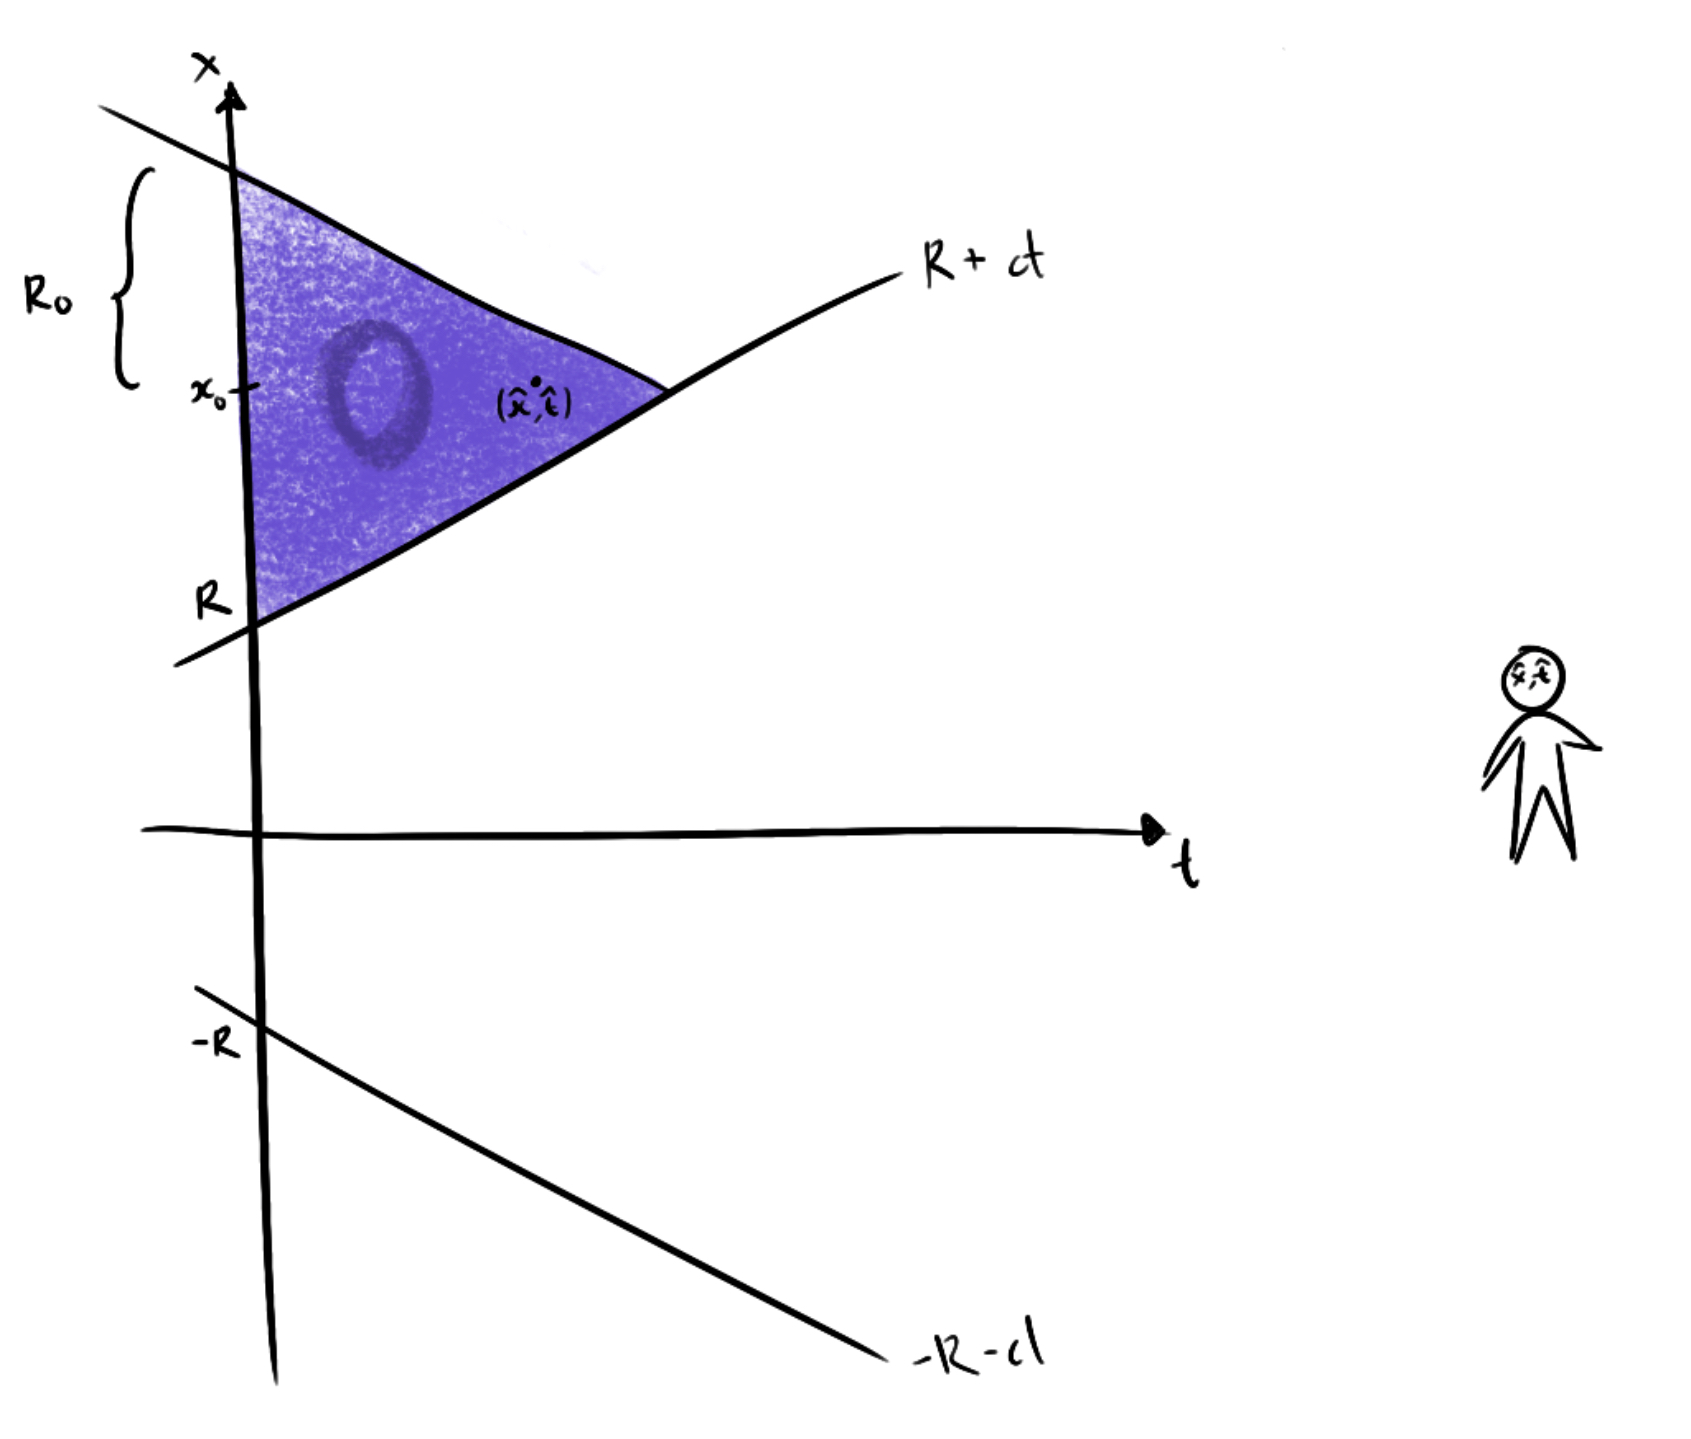
\includegraphics[height=6.5cm]{../images/0void2}
    \end{center}

    \item We have done this in class, but we can repeat the derivation. Let $t_0 < R_0/c_2$. Suppose $u, u'$ are two solutions to the PDE in $[0, t_0] \times \RR$. Note that the notation $u'$ is not to be confused with a derivative of $u$. Consider $v=u -u'$. We see that 
    \[v_{tt} - \D \cdot (c^2 \D v) +qv =  u_{tt} - \D \cdot (c^2 \D u) +qu - u'_{tt} + \D \cdot (c^2 \D u') -qu' = 0 - 0 = 0.\]
    Moreover, 
    \[v(x,0) = u(x,0) - u'(x,0)= \phi(x)- \phi(x)=0\]
    and 
    \[v_t(x,0) = u_t(x,0) - u'_t(x,0)= \psi(x)- \psi(x)=0.\]
    So, we see that $v$ satisfies the same equation with 0 initial conditions. If we define $E$ as in part (a), but for $v$, we see that for any $x_0,$ the initial conditions give us 
    \[E(0) = 0.\]
    Since $E(t)$ is non-increasing and non-negative, we know that 
    \[E(t) = 0\]
    for all $t \in [0,t_0]$. As in part (b), this means that $v_x$ and $v_t$ vanish where $|x - x_0| < R_0-c_t$. So, $v$ vanishes on this region as well. For any $(t,x) \in [0,t_0] \times \RR$, we can select $x_0 = x$ and see that the point is in the region where $v =0$. Thus,  $v = 0$ on all of $[0,t_0] \times \RR$. 
    \hop 
    So, we can conclude that $u = u'$, and the solution is unique. \qed

\end{enumerate}

\end{document}